\section[1998年高考数学试卷及答案(全国卷)理科]{1998年普通高等学校招生考试(全国卷)\\\Huge{理科数学}}

\begin{questions}
	\question $\sin\ang{600}$的值是 \hfs

	\begin{oneparchoices}
		\choice $\frac12$
		\choice $-\frac12$
		\choice $\frac{\sqrt{3}}{2}$
		\CorrectChoice $-\frac{\sqrt{3}}{2}$
	\end{oneparchoices}

	\begin{solution}
		\begin{align*}
			\sin\ang{600} = \sin\ang{240} = -\frac{\sqrt{3}}{2}
		\end{align*}
	\end{solution}

	\question 函数$y=a^{|x|}(a>1)$的图像是\hfs

	\begin{oneparchoices}
		\choice
		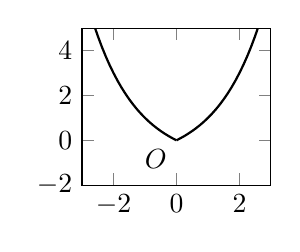
\begin{tikzpicture}
			\begin{axis}[
					domain = -3:3,
					ymin = -2,
					ymax = 5,
					scale=.35
				]
				\addplot[thick, domain=0:3]{2^x - 1};
				\addplot[thick, domain=-3:0]{2^(-x) - 1};
				\node[below left] at(0,0) {$O$};
			\end{axis}
		\end{tikzpicture}
		\CorrectChoice
		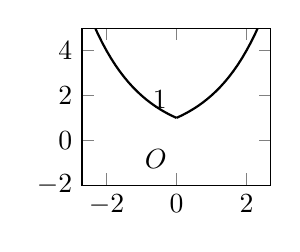
\begin{tikzpicture}
			\begin{axis}[
					domain = -3:3,
					ymin = -2,
					ymax = 5,
					scale=.35
				]
				\addplot[thick, domain=0:3]{2^x};
				\addplot[thick, domain=-3:0]{2^(-x)};
				\node[below left] at(0,0) {$O$};
				\node[above left] at(0,1) {$1$};
			\end{axis}
		\end{tikzpicture}

		\choice
		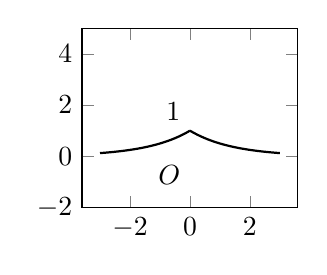
\begin{tikzpicture}
			\begin{axis}[
					domain = -3:3,
					ymin = -2,
					ymax = 5,
					scale=.4
				]
				\addplot[thick, domain=0:3]{2^(-x)};
				\addplot[thick, domain=-3:0]{2^(x)};
				\node[below left] at(0,0) {$O$};
				\node[above left] at(0,1) {$1$};
			\end{axis}
		\end{tikzpicture}

		\choice
		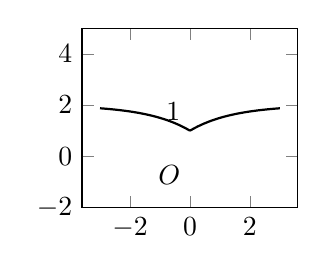
\begin{tikzpicture}
			\begin{axis}[
					domain = -3:3,
					ymin = -2,
					ymax = 5,
					scale=.4
				]
				\addplot[thick, domain=0:3]{2-2^(-x)};
				\addplot[thick, domain=-3:0]{2-2^(x)};
				\node[below left] at(0,0) {$O$};
				\node[above left] at(0,1) {$1$};
			\end{axis}
		\end{tikzpicture}
	\end{oneparchoices}

	\begin{solution}
		$a^{|x|} (a>1)$的最小值是$1$,而且不收敛,所以答案是B.
	\end{solution}

	\question 曲线的极坐标方程$\rho=4\sin\theta$化成直角坐标方程为 \hfs

	\begin{oneparchoices}
		\choice $x^2 + (y+2)^2 = 4$ \CorrectChoice $x^2 + (y-2)^2 = 4$
		\choice $(x-2)^2 + y^2 = 4$ \choice $(x+2)^2 + y^2 = 4$
	\end{oneparchoices}
	\begin{solution}
		设曲线上的动点$P(x,y)$,则有:
		\begin{align*}
			y    & = \rho\sin\theta                 \\
			x    & = \rho\cos\theta                 \\
			\rho & = \sqrt{x^2 + y^2} = 4\sin\theta
		\end{align*}
		则有
		\begin{align*}
			\sqrt{x^2 + y^2} & = 4\frac{y}{\rho} \\
			x^2 + y^2        & = 4y              \\
			x^2 + (y-2)^2    & = 4
		\end{align*}
	\end{solution}

	\question 两条直线$A_1x + B_1y + C_1 = 0, A_2x + B_2y + C_2=0$垂直的充要条件是 \hfill(\hspace{1cm})

	\begin{oneparchoices}
		\CorrectChoice $A_1A_2 + B_1B_2 =0$ \choice $A_1A_2 - B_1B_2 = 0$ \choice $\dfrac{A_1A_2}{B_1B_2} = -1$
		\choice $\dfrac{A_1A_2}{B_1B_2} = 1$
	\end{oneparchoices}

	\begin{solution}
		直线的斜率分别为$-\dfrac{A_1}{B_1}$和$-\dfrac{A_2}{B_2}$,两条直线垂直的充要条件是斜率的乘积为$-1$,所以答案选择A.
	\end{solution}

	\question 函数$f(x)=\frac1x(x\neq0)$的反函数$f^{-1}(x)=$ \hfs

	\begin{oneparchoices}
		\choice $x ( x\neq0)$ \CorrectChoice $\frac1x(x\neq0)$ \choice $-x (x\neq0)$ \choice $-\frac1x (x\neq0)$
	\end{oneparchoices}
	\begin{solution}
		因为$y=\frac1x$关于$y=x$对称,所以反函数是其本身.
	\end{solution}

	\question 已知点$P(\sin\alpha-\cos\alpha, \tan\alpha)$在第一象限,则在$[0,2\pi]$内$\alpha$的取值范围是 \hfill
	(\hspace{1cm})

	\begin{choices}
		\choice $\left( \dfrac{\pi}{2}, \dfrac{3\pi}{4} \right) \cup \left( \pi, \dfrac{5\pi}{4} \right)$
		\CorrectChoice $\left( \dfrac{\pi}{4}, \dfrac{\pi}{2} \right) \cup \left( \pi, \dfrac{5\pi}{4} \right)$
		\choice $\left( \dfrac{\pi}{2}, \dfrac{3\pi}{4} \right) \cup \left( \dfrac{5\pi}{4}, \dfrac{3\pi}{2} \right)$
		\choice $\left( \dfrac{\pi}{4}, \dfrac{\pi}{2} \right) \cup \left( \dfrac{3\pi}{4}, \pi \right)$
	\end{choices}

	\begin{solution}
		根据条件有:
		\begin{align*}
			\sin\theta - \cos\theta > 0 \tag{a} \\
			\tan\theta = \frac{\sin\theta}{\cos\theta} > 0 \tag{b}
		\end{align*}
		根据式$(a)$有$\alpha \in \left( \dfrac{\pi}{4}, \dfrac{5\pi}{4} \right)$;根据式$(b)$有$\alpha \in \left( 0,
			\dfrac{\pi}{2} \right) \cup \left( \pi, \dfrac{3\pi}{2} \right)$

		综上可得取值范围为B.
	\end{solution}

	\question 已知圆锥的全面积是底面积的$3$倍,那么该圆锥的侧面展开图扇形的圆心角为\hfs

	\begin{oneparchoices}
		\choice $\ang{120}$
		\choice $\ang{150}$
		\CorrectChoice $\ang{180}$
		\choice $\ang{240}$
	\end{oneparchoices}

	\begin{solution}
		设圆锥的底面半径为$r$,棱线长为$l$,则底面积为$\pi r^2$,侧面积为$\frac{2\pi r}{2\pi l}\pi l^2 = \pi
			rl$,由题意有$\pi rl = 2\pi r^2$,即$l=2r$,展开图的圆心角为$2\pi\frac{r}{l}=\pi$,选C.
	\end{solution}

	\question 复数$-i$的一个立方根是$i$,它的另外两个立方根是 \hfs

	\begin{oneparchoices}
		\choice $\dfrac{\sqrt{3}}{2} \pm \dfrac12i$
		\choice $-\dfrac{\sqrt{3}}{2} \pm \dfrac12i$
		\choice $\pm\dfrac{\sqrt{3}}{2} + \dfrac12i$
		\CorrectChoice $\pm\dfrac{\sqrt{3}}{2} - \dfrac12i$
	\end{oneparchoices}

	\begin{solution}
		根据欧拉恒等式$e^{i\theta} = \cos\theta + i\sin\theta$,当$\theta=\frac32\pi$时有$e^{i\frac32\pi} =
			-i$.其立方根为$e^{i(\frac{\frac32\pi + 2k\pi}{3})}, (k=0,1,2)$.

		\begin{cenum}
			\item 当$k=0$时,$e^{\frac12\pi} = \cos \left( \dfrac12\pi \right) + \sin \left( \dfrac12\pi \right)i = i$
			\item 当$k=1$时,$e^{\frac76\pi} = \cos \left( \dfrac76\pi \right) + \sin \left( \dfrac76\pi \right)i =
				      -\frac{\sqrt{3}}{2} - \frac12i$
			\item 当$k=2$时,$e^{\frac{11}6\pi} = \cos \left( \dfrac{11}6\pi \right) + \sin \left( \dfrac{11}6\pi \right)i =
				      \frac{\sqrt{3}}{2} - \frac12i$
		\end{cenum}
		答案选D.
	\end{solution}

	\question 如果棱台的两底面积分别是$S,S'$,中截面的面积是$S_0$,那么 \hfs

	\begin{oneparchoices}
		\CorrectChoice $2\sqrt{S_0} = \sqrt{S} + \sqrt{S'}$
		\choice $S_0 = \sqrt{SS'}$
		\choice $2S_0 = S + S'$
		\choice $S_0^2 = 2SS'$
	\end{oneparchoices}

	\begin{solution}
		一维方向上有 $\sqrt{S_0} = \frac{\sqrt{S} + \sqrt{S'}}{2}$,所以选择A.
	\end{solution}

	\question 向高为$H$的水瓶中注水,注满为止,如果注水量$V$与水深$h$的函数关系的图像如下图所示,那么水瓶的形状是 \hfs

	\begin{center}
		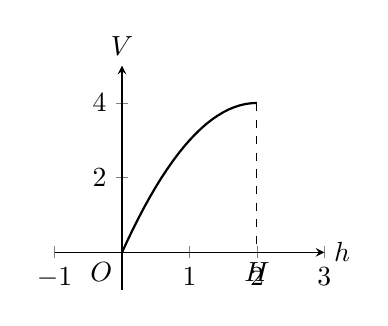
\begin{tikzpicture}
			\begin{axis}[
					axis lines=middle,
					xlabel = $h$,
					ylabel = $V$,
					xlabel style = {anchor=west},
					ylabel style = {anchor=south},
					ymin = -1,
					ymax = 5,
					xmax = 3,
					xmin = -1,
					scale = .5
				]
				\addplot[thick, domain=0:2]{-x^2+ 4*x};
				\node[below left] at(0,0) {$O$};
				\draw [dashed] (2,4)  -- (2,0) node[below]{$H$};
			\end{axis}
		\end{tikzpicture}
	\end{center}

	\tdplotsetmaincoords{80}{0}
	\begin{oneparchoices}
		\choice
		\begin{tikzpicture}[tdplot_main_coords, scale=.5]
			\tkzDefPoints{0/0/O, 1/0/A, -1/0/B}
			\coordinate(O') at (0,0,4);
			\coordinate(A') at (2,0,4);
			\coordinate(B') at (-2,0,4);

			\tkzDrawSegments(A,A' B,B')
			\tkzDrawSemiCircle(O',A')
			\tkzDrawSemiCircle(O',B')

			\tkzDrawSemiCircle[dashed](O,A)
			\tkzDrawSemiCircle(O,B)
		\end{tikzpicture}

		\CorrectChoice
		\begin{tikzpicture}[tdplot_main_coords, scale=.5]
			\tkzDefPoints{0/0/O, 2/0/A, -2/0/B}
			\coordinate(O') at (0,0,4);
			\coordinate(A') at (1,0,4);
			\coordinate(B') at (-1,0,4);

			\tkzDrawSegments(A,A' B,B')
			\tkzDrawSemiCircle(O',A')
			\tkzDrawSemiCircle(O',B')

			\tkzDrawSemiCircle[dashed](O,A)
			\tkzDrawSemiCircle(O,B)
		\end{tikzpicture}

		\choice
		\begin{tikzpicture}[tdplot_main_coords, scale=.5]
			\tkzDefPoints{0/0/O, 2/0/A, -2/0/B}
			\coordinate(O') at (0,0,4);
			\coordinate(A') at (2,0,4);
			\coordinate(B') at (-2,0,4);
			\coordinate(C) at (3.5,0, 2);
			\coordinate(C') at (-3.5,0, 2);

			\draw[very thin](A) to[out=120, in=240](A');
			\draw[very thin](B) to[out=60, in=300](B');
			% \tkzDrawSegments(A,C C,A' B,C' C',B')
			% \draw[very thin](A)  .. controls ($(C)-(1.3,0,2)$) and ($(C)-(1.3,0,2)$) .. (A');
			\tkzDrawSemiCircle(O',A')
			\tkzDrawSemiCircle(O',B')

			\tkzDrawSemiCircle[dashed](O,A)
			\tkzDrawSemiCircle(O,B)
		\end{tikzpicture}

		\choice
		\begin{tikzpicture}[tdplot_main_coords, scale=.5]
			\tkzDefPoints{0/0/O, 2/0/A, -2/0/B}
			\coordinate(O') at (0,0,4);
			\coordinate(A') at (2,0,4);
			\coordinate(B') at (-2,0,4);

			\tkzDrawSegments(A,A' B,B')
			\tkzDrawSemiCircle(O',A')
			\tkzDrawSemiCircle(O',B')

			\tkzDrawSemiCircle[dashed](O,A)
			\tkzDrawSemiCircle(O,B)
		\end{tikzpicture}
	\end{oneparchoices}

	\begin{solution}
		由函数图像可以看出斜率是逐渐下降的,所以选择B.
	\end{solution}

	\question $3$名医生和$6$名护士被分配到$3$所学校为学生体检,每校分配$1$名医生和$2$名护士,不同的分配方法共有

	\hfs

	\begin{oneparchoices}
		\choice $90$种
		\choice $180$种
		\choice $270$种
		\CorrectChoice $540$种
	\end{oneparchoices}

	\begin{solution}
		$3$名医生分到三个学校共有$3!=6$种分配方法.

		$6$名护士分到三个学校,每个学校两名护士有$\displaystyle\binom{6}{2}\cdot\binom{4}{2}\cdot\binom{2}{2}=90$种分配方法.

		所以总共有$6\times90=540$种分配方法.
	\end{solution}

	\question 椭圆$\dfrac{x^2}{12} + \dfrac{y^2}{3} =
		1$的焦点为$F_1$和$F_2$,点$P$在椭圆上,如果线段$PF_1$的中点在$y$轴上,那么$|PF_1|$是$|PF_2|$的

	\hfs

	\begin{oneparchoices}
		\CorrectChoice $7$倍
		\choice $5$倍
		\choice $4$倍
		\choice $3$倍
	\end{oneparchoices}

	\begin{solution}
		$c=\sqrt{12-3} = 3$,所以焦点分别为$(-3,0), (3,0)$.

		如果$PF_1$的中点在$y$轴上,则可知$P$点的$x$坐标为$3$.此时$\triangle{F_1F_2P}$是一个直角三角形,其中$|F_1F_2|=6$,$|PF_2|=\dfrac{\sqrt{3}}{2}$,则$|PF_1|=\sqrt{6^2+\frac{3}{4}}=\frac72\sqrt{3}$,所以答案选A.
	\end{solution}

	\question
	球面上有$3$个点,其中任意两点的球面距离都等于大圆周长的$\frac16$,经过这$3$个点的小圆的周长为$4\pi$,那么这个球的半径为
	\hfs

	\begin{oneparchoices}
		\choice $4\sqrt{3}$
		\CorrectChoice $2\sqrt{3}$
		\choice $2$
		\choice $\sqrt{3}$
	\end{oneparchoices}

	\begin{solution}
		经过三个点的小圆的周长为$4\pi$,则小圆的半径$r=2$.则可进一步推算出小圆内接等边三角形的边长为$2\sqrt{3}$.因为任意两点的球面距离是大圆的周长的$\frac16$,所以两个点之间的夹角为$\ang{60}$,因此球心与其中两个点的组成一个等边三角形,所以球的半径等于两点之间的距离$2\sqrt{3}$.
	\end{solution}

	\question 一个直角三角形三内角的正弦值成等比数列,其最小内角为\hfs

	\begin{oneparchoices}
		\choice $\arccos\dfrac{\sqrt{5}-1}{2}$
		\CorrectChoice $\arcsin\dfrac{\sqrt{5}-1}{2}$
		\choice $\arccos\dfrac{1-\sqrt{5}}{2}$
		\choice $\arcsin\dfrac{1-\sqrt{5}}{2}$
	\end{oneparchoices}

	\begin{solution}
		根据正弦定理有$\frac{\sin A}{a}=\frac{\sin B}{b}=\frac{\sin C}{c}$,所以三条边也成等比数列.
		\begin{equation*}
			\frac{a}{b} = \frac{b}{c} \tag{1}
		\end{equation*}
		又因为三角形是直角三角形,所以有
		\begin{equation*}
			a^2 + b^2 = c^2 \tag{2}
		\end{equation*}
		将式$(1)$转化为$b^2=ac$并代入式$(2)$可得:
		\begin{equation*}
			a^2 + ac = c^2
		\end{equation*}
		两边都除以$ac$得:
		\begin{equation*}
			\frac{a}{c} + 1 = \frac{c}{a}
		\end{equation*}

		设$\sin{A}=\frac{a}{c}=x$则原式可以表示为:
		\begin{align*}
			x + 1 = \frac{1}{x} \\
			x^2 + x - 1 = 0     \\
			x_1,x_2 = \frac{-1\pm\sqrt{5}}{2}
		\end{align*}
		因为$\angle{A}<\ang{90}$,所以$\sin{A}=\frac{-1+\sqrt{5}}{2}$,所以$\angle{A}$可以表示为$\arcsin{\frac{-1+\sqrt{5}}{2}}$.
	\end{solution}

	\question 在等比数列${a_n}$中,$a_1>1$,且前$n$项和$S_n$满足$\displaystyle
		\lim_{n\to\infty}S_n=\frac{1}{a_1}$,那么$a_1$的取值范围是 \hfs

	\begin{oneparchoices}
		\choice $(1,+\infty)$
		\choice $(1,4)$
		\choice $(1,2)$
		\CorrectChoice $(1,\sqrt{2})$
	\end{oneparchoices}

	\begin{solution}
		\begin{align*}
			\lim_{n\to\infty}S_n & = \lim_{n\to\infty}a_1\frac{1-q^n}{1-q} \\
			                     & = a_1\frac{1}{1-q}\qquad (|q|< 1)       \\
			                     & = a_1
		\end{align*}
		整理得:
		\begin{equation*}
			a_1^2 = 1 - q \qquad (|q|<1)
		\end{equation*}
		则有$0<a_1^2<2$,结合题中$a_1>1$可得$a_1$的取值范围为$(1,\sqrt{2})$.
	\end{solution}

	\question 设圆过双曲线$\frac{x^2}{9} -
		\frac{y^2}{16}=1$的一个顶点和一个焦点,圆心在此双曲线上,则圆心到双曲线中心的距离是\fillin[$\frac{16}{3}$][2cm].

	\begin{solution}
		双曲线的顶点为$(-3,0)$和$(3,0)$,焦点为$(-5,0)$和$(5,0)$,由圆的特性可知圆心必在过顶点和焦点中心的垂直线上.这样可以推断出圆是过同一侧的顶点和焦点,因为如果不在同一侧,中心线分别为$x=\pm1$,与双曲线没有交点.

		那么可以考察右侧的顶点和焦点,则圆心在$x=4$上,代入双曲线方程可以计算得$y^2=\dfrac{112}{9}$,则圆心到双曲线中心$(0,0)$的距离为:
		\begin{align*}
			\sqrt{x^2 + y^2} & = \sqrt{4^2 + \frac{112}{9}} \\
			                 & = \frac{16}{3}
		\end{align*}
	\end{solution}

	\question $(x+2)^{10}(x^2-1)$的展开式中$x^{10}$的系数为\fillin[179][2cm].(用数字作答)

	\begin{solution}
		根据二项式定理$(x+2)^{10}$可以展开为
		\begin{equation*}
			\sum_{n=0}^{10}\binom{10}{n}x^{10-n}2^{n}
		\end{equation*}
		则有$x^{10}$的系数为$1$,$x^8$的系数为$\binom{10}{2}2^2 =
			180$,再乘以$(x^2-1)$后原来的$x^{10}$的系数变为$-1$,原来$x^8$变为$x^{10}$,系数为$180$不变,则有展开式的$x^{10}$的系数为$179$.
	\end{solution}

	\question 在直四棱柱$A_1B_1C_1D_1-ABCD$中,当底面四边形$ABCD$满足条件\fillin[正方形或菱形][2cm]时,有$A_1C\perp
		B_1D_1$.(注:填上你认为正确的一种条件即可,不必考虑所有可能的情形)

	\begin{solution}
		\tdplotsetmaincoords{60}{110}
		\begin{tikzpicture}[tdplot_main_coords]
			\tkzDefPoints{0/0/A,2/0/B,2/2/C,0/2/D}
			\coordinate (A1) at (0,0,4);
			\coordinate (B1) at (2,0,4);
			\coordinate (C1) at (2,2,4);
			\coordinate (D1) at (0,2,4);

			\tkzDrawPolygon(A1,B1,C1,D1)
			\tkzDrawSegments(B,B1 C,C1 D,D1 B,C C,D)
			\tkzDrawSegments[dashed](A,A1 B,A A,D A1,C)

			\tkzLabelPoints(A,B,C,D)
			\tkzLabelPoints[above](A1,B1,C1,D1)

			\tkzDrawSegments(B1,D1 A1,C1)

		\end{tikzpicture}
		可以看到$A_1C$在四边形$A_1B_1C_1D_1$上的投影为$A_1C_1$,如果$A_1C_1 \perp B_1D_1$,则有$A_1C \perp
			B_1D_1$,所以底面四边形$ABCD$如果是正方形或者菱形即可.
	\end{solution}

	\question 关于函数$f(x)=4\sin \left( 2x + \dfrac{\pi}{3} \right)\quad (x\in \mathbf{R})$,有下列命题:
	\begin{enumerate}[label=\protect\circled{\arabic*}]
		\item 由$f(x_1) = f(x_2) = 0$可得$x_1 - x_2$必是$\pi$的整数倍;
		\item $y=f(x)$的表达式可改写为$y=4\cos \left( 2x - \dfrac{\pi}{6} \right)$;
		\item $y=f(x)$的图像关于点$\left( -\dfrac{\pi}{6}, 0\right)$对称;
		\item $y=f(x)$的图像关于直线$x=-\dfrac{\pi}{6}$对称.
	\end{enumerate}
	其中正确的命题的序号是\fillin[\circled{2}、\circled{3}][2cm].(注:把你认为正确的序号都填上)

	\begin{solution}
		\begin{enumerate}[label=\protect\circled{\arabic*}]
			\item 由$f(x_1) = f(x_2) = 0$可知$2x_1 + \frac{\pi}{3} - 2x_2 - \frac{\pi}{3} = 2(x_1-x_2) =
				      k\pi$,所以$x_1-x_2=\frac{k}{2}\pi$  \textcolor{red}{\times}
			\item $y=4\sin \left( 2x + \dfrac{\pi}{3} \right)=4\cos \left( \dfrac{\pi}{2} - 2x - \dfrac{\pi}{3} \right)
				      = 4\cos \left( \dfrac{\pi}{6} - 2x \right) = 4\cos \left( 2x - \dfrac{\pi}{6} \right)$ \textcolor{red}{\checkmark}
			\item 如图,所以\circled{3}正确、\circled{4}错误.

			      \begin{center}
				      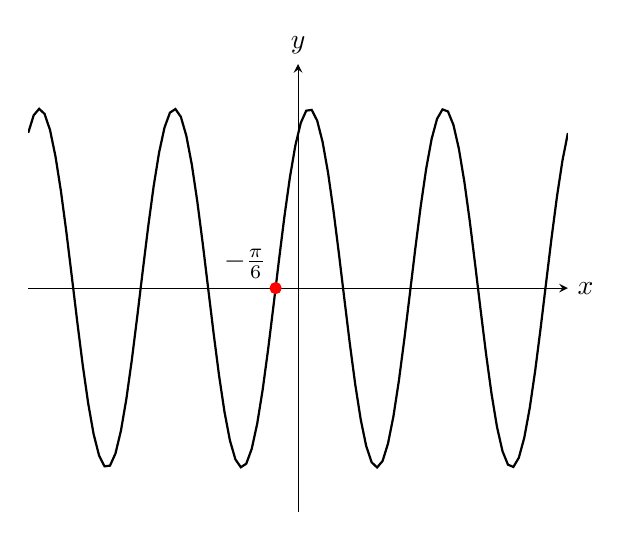
\begin{tikzpicture}
					      \begin{axis}[
							      axis lines=middle,
							      xlabel = $x$,
							      ylabel = $y$,
							      xlabel style={right},
							      ylabel style={above},
							      ymax = 5,
							      ymin = -5,
							      samples = 100,
							      ticks = none
						      ]
						      \addplot[thick, domain=-2*pi:2*pi]{4*sin(deg(2*x + pi/3))};
						      \draw[draw=red, fill=red]({-pi/6}, 0)node[above left]{$-\frac{\pi}{6}$}circle(2pt);
					      \end{axis}

				      \end{tikzpicture}
			      \end{center}

		\end{enumerate}
	\end{solution}
	\question 在$\triangle{ABC}$中,$a$,$b$,$c$分别是角$A,B,C$的对边,设$a+c=2b,
		A-C=\dfrac{\pi}{3}$,求$\sin{B}$的值.

	\begin{solution}
		由正弦定理有$\dfrac{a}{\sin{A}}=\dfrac{b}{\sin{B}}=\dfrac{c}{\sin{C}}$和题中的$a+c=2b$可得:
		\begin{equation*}
			\sin{A} + \sin{C} = 2\sin{B}
		\end{equation*}
		由和差化积公式$\sin\alpha + \sin\beta = 2\sin{\dfrac{\alpha+\beta}{2}}\cos{\dfrac{\alpha-\beta}{2}}$可得:
		\begin{align*}
			\sin{A} + \sin{C} & = 2\sin \left( \frac{A+C}{2} \right)\cos \left( \frac{A-C}{2} \right) \\
			                  & = 2\sin \left( \frac{A+C+B - B}{2} \right) \cos{\frac{\pi}{6}}        \\
			                  & = \sqrt{3}\sin(\ang{90}-\frac{B}{2})                                  \\
			                  & = \sqrt{3}\cos\left(\frac{B}{2}\right)
		\end{align*}
		又因为$\sin{B}=2\sin\left(\dfrac{B}{2}\right)\cos\left(\dfrac{B}{2}\right)$,代入得:
		\begin{align*}
			4\sin\left(\frac{B}{2}\right)\cos\left(\frac{B}{2}\right) = \sqrt{3}\cos\left(\frac{B}{2}\right) \\
			\sin\left(\frac{B}{2}\right) = \frac{\sqrt{3}}{4}
		\end{align*}
		因为$\frac{B}{2}$肯定为锐角,所以
		\begin{equation*}
			\cos\left(\frac{B}{2}\right) = \sqrt{1 - \sin^2 \left(\frac{B}{2}\right)}= \frac{\sqrt{13}}{4}
		\end{equation*}
		则有:
		\begin{equation*}
			\sin{B} = 2\sin{\left( \frac{B}{2} \right)} \cos{\left( \frac{B}{2}
				\right)}=2\cdot\frac{\sqrt{3}}{4}\cdot\frac{\sqrt{13}}{4} = \frac{\sqrt{39}}{8}
		\end{equation*}
	\end{solution}

	\question 如图,直线$l_1$和$l_2$相交于点$M$,$l_1 \perp l_2$,点$N\in
		l_1$.以$A,B$为端点的曲线段$C$上的任一点到$l_2$的距离与点$N$的距离相等.若$\triangle{AMN}$为锐角三角形,$|AM|=\sqrt{17},|AN|=3,$且$|BN|=6$.建立适当的坐标系,求曲线$C$的方程.
	\begin{figure*}[htbp]
		\centering
		\begin{tikzpicture}[scale=0.5]
			\tkzDefPoints{0/0/M, 3/0/N, 0/3/P}
			\tkzDefPoint(40:{sqrt(17)}){A}
			\tkzDefPoint(6,5){B}
			\tkzInit[xmin=-2, xmax=6]
			\tkzDrawX

			\tkzDefLine[orthogonal=through A](M,P) \tkzGetPoint{x}
			\tkzInterLL(M,P)(A,x) \tkzGetPoint{D}

			\tkzDrawSegments[add=.5 and .5](M,N M,P)
			\tkzDrawSegments(A,M A,N B,N)
			\draw[shorten >= -1cm , shorten <= -1cm, -Latex] ([xshift=1.5cm]M) --([xshift=1.5cm]P) node[above=1cm]{$y$};
			\draw[very thin] (A) .. controls (4,5) and (5.5,5) .. (B);
			\tkzDrawSegment[dashed](A,D)

			\tkzLabelSegment[right=1.5cm, below](M,N){$l_1$}
			\tkzLabelSegment[above=1.5cm](M,P){$l_2$}
			\tkzLabelPoint[below left](M){$M$}
			\tkzLabelPoint[below](N){$N$}
			\tkzLabelPoint[above left](A){$A$}
			\tkzLabelPoint[above right](B){$B$}
			\tkzLabelPoint[left](D){$D$}
		\end{tikzpicture}
	\end{figure*}

	\begin{solution}
		\begin{enumerate}[label=\protect\circled{\arabic*}]
			\item 以$l_1$为$x$轴,过$MN$的中线为$y$轴,设抛物线的方程为$x=\dfrac{y^2}{4p}$.
			\item 过$A$点作垂线到$l_2$,垂足为$D$
			      \begin{align*}
				       & \because AD = AN = 3                                                  \\
				       & \therefore A \text{点横坐标为} 3-p                                         \\
				       & \therefore  |DM| = \sqrt{|AM|^2 - |DA|^2} = \sqrt{17 - 9} = 2\sqrt{2} \\
				       & \therefore A\text{点的纵坐标为}2\sqrt{2}                                    \\
			      \end{align*}
			\item 将$A$点坐标$(3-p, 2\sqrt{2})$代入抛物线方程得:
			      \begin{align*}
				      3-p = \frac{(2\sqrt{2})^2}{4p} \\
				      p^2 -3p + 2 = 0                \\
				      (p-2)(p-1) = 0
			      \end{align*}
			      则有$p_1 = 1, p_2 = 2$
			\item 当$p=1$时,$MN=2$,此时有$|AM|^2 > |AN|^2 +
				      |MN|^2$,可以判定$\triangle{AMN}$是钝角三角形,与条件不符,所以$p=2$,即曲线的方程为$x=\dfrac{y^2}{8}$.
			\item 根据题意可知$B$点的横坐标为$6-p=4$,代入曲线方程得:
			      \begin{align*}
				      4 = \frac{y^2}{8}
				      y = \pm4\sqrt{2}
			      \end{align*}
			      因为曲线段$C$在第一象限,所以$B$点坐标为$(4,4\sqrt{2})$

			\item 综上,曲线的方程为:
			      \begin{equation*}
				      x = \frac{y^2}{8} \quad (1 \leqslant x \leqslant 4, y>0)
			      \end{equation*}
		\end{enumerate}

	\end{solution}

	\question
	如图,为处理含有某种杂质的污水,要制造一底宽为$2$米的均长方体沉淀箱,污水从$A$孔流入,经沉淀后从$B$孔流出.设箱体的长度为$a$米,调试为$b$米.已知流出的水中该杂质的质量分数与$a,b$的乘积$ab$成反比.现有制箱材料$60$平方米.问当$a,b$各为多少米时,经沉淀后流出的水路该杂质的质量分数最小.($A$、$B$孔的面积忽略不计)

	\begin{figure*}[ht]
		\centering
		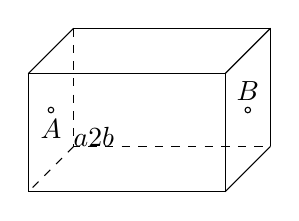
\begin{tikzpicture}[scale=.5]
			\coordinate(A) at (0,0);
			\coordinate(B) at (5,0);
			\coordinate(C) at (5,3);
			\coordinate(D) at (0,3);
			\coordinate(A') at (0,0,3);
			\coordinate(B') at (5,0,3);
			\coordinate(C') at (5,3,3);
			\coordinate(D') at (0,3,3);

			\draw [dashed](D) -- (A) -- (B) ;
			\draw (B)	-- (C) -- (D);
			\draw (A') -- (B') -- (C') -- (D')--cycle;
			\draw[dashed](A) -- (A');
			\draw(B) -- (B');
			\draw(C) -- (C');
			\draw(D) -- (D');

			\draw (0,1.5,1.5) circle (2pt);
			\draw (5,1.5,1.5) circle (2pt);
			\node[below] at(0,1.5,1.5) {$A$};
			\node[above] at(5,1.5,1.5) {$B$};

			\tkzLabelSegment(A',B'){$a$}
			\tkzLabelSegment(B,B'){$2$}
			\tkzLabelSegment[left](C',B'){$b$}
		\end{tikzpicture}
	\end{figure*}

	\begin{solution}
		根据总面积为$60$平方米可得如下关系:
		\begin{equation*}
			60 = 2a + 2ab + 4b
		\end{equation*}
		化简得:
		\begin{equation*}
			30 = a + ab + 2b \tag{a}
		\end{equation*}
		设$y=ab$,则有$b=\frac{y}{a}$,代入上面的式子中可得:
		\begin{align*}
			30 = a + y + \frac{2}{a}y           \\
			(1+\frac2a)y = 30 - a               \\
			y = \frac{30-a}{1 + \frac2a}        \\
			y = \frac{a(30-a)}{a+2}     \tag{b} \\
		\end{align*}
		\subsection*{解法一}
		对式$(b)$求导:
		\begin{align*}
			y' & = \left( \frac{a(30-a)}{a+2} \right)'              \\
			   & = \frac{(30-2a)(a+2) - a(30-a)}{(a+2)^2}           \\
			   & = \frac{30a + 60 - 2a^2 - 4a - 30a + a^2}{(a+2)^2} \\
			   & = \frac{60 - 4a - a^2}{(a+2)^2}                    \\
			   & = \frac{(10+a)(6-a)}{(a+2)^2}
		\end{align*}
		因为$a>0$,所以只有$a=6$时$y'=0$,即此时$y=ab$有最大值.将$a=6$代入面积关系式$(a)$中可得:
		\begin{equation*}
			30 = 6 + 6b + 2b
		\end{equation*}
		解得$b=3$米.

		综上,当$a=6$米、$b=3$米时质量分数最小.

		\subsection*{解法二}
		化简式$(b)$:
		\begin{align*}
			y & = \frac{30a -a^2}{a+2}                      \\
			  & = \frac{30a + 4 + 4a - (4 + 4a + a^2)}{a+2} \\
			  & = \frac{34a + 4 - (a+2)^2}{a+2}             \\
			  & = \frac{34(a+2) -64 - (a+2)^2}{a+2}         \\
			  & = 34 - \frac{64}{a+2} - (a+2)               \\
		\end{align*}
		$\dfrac{64}{a+2} + (a+2) \geqslant 2\sqrt{\dfrac{64}{a+2}\cdot(a+2)} = 16$,当且仅当$\dfrac{64}{a+2} =
			a+2$时有最小值,即$(a+2)^2 = 64$,因为$a>0$所以$a=6$,代入式$(a)$中求得$b=3$.
	\end{solution}

	\question
	已知斜三棱柱$ABC-A_1B_1C_1$的侧面$A_1ACC_1$与底面$ABC$垂直,$\angle{ABC}=\ang{90}$,$BC=2,AC=2\sqrt{3}$,且$AA_1
		\perp A_1C, AA_1=A_1C$.
	\begin{penum}
		\item 求侧棱$A_1A$与底面$ABC$所成角的大小;
		\item 求侧面$A_1ABB_1$与底面$ABC$所成二面角的大小;
		\item 求顶点$C$到侧面$A_1ABB_1$的距离.
	\end{penum}
	\begin{figure*}[ht]
		\centering
		\tdplotsetmaincoords{60}{140}
		\begin{tikzpicture}[tdplot_main_coords, scale=2]
			\coordinate (A) at ({2*sqrt(3)},0);
			\coordinate (B) at (25:2);
			\coordinate (C) at (0,0);
			\coordinate (A1) at ({2*sqrt(3)-2},0,2);
			\coordinate (B1) at (B);
			\path (B1) ++(-2,0,2) coordinate (B1);
			\coordinate (C1) at (-2,0,2);

			\tkzDrawSegments(A,B B,C C,C1 C1,A1 A1,B1 B1,B A1,A B1,C1)
			\tkzDrawSegments[dashed](A,C A1,C)

			\tkzLabelPoints(A,B,C)
			\tkzLabelPoint[left](A1){$A_1$}
			\tkzLabelPoint[above](B1){$B_1$}
			\tkzLabelPoint[right](C1){$C_1$}

		\end{tikzpicture}
	\end{figure*}

	\begin{solution}
		\begin{center}
			\tdplotsetmaincoords{60}{140}
			\begin{tikzpicture}[tdplot_main_coords, scale=2]
				\coordinate (A) at ({2*sqrt(3)},0);
				\coordinate (B) at (25:2);
				\coordinate (C) at (0,0);
				\coordinate (A1) at ({2*sqrt(3)-2},0,2);
				\coordinate (B1) at (B);
				\path (B1) ++(-2,0,2) coordinate (B1);
				\coordinate (C1) at (-2,0,2);

				\tkzDrawSegments(A,B B,C C,C1 C1,A1 A1,B1 B1,B A1,A B1,C1)
				\tkzDrawSegments[dashed](A,C A1,C)

				\tkzLabelPoints(A,B,C)
				\tkzLabelPoint[left](A1){$A_1$}
				\tkzLabelPoint[above](B1){$B_1$}
				\tkzLabelPoint[right](C1){$C_1$}

				\tkzMarkRightAngle[blue](C,B,A)
				\tkzMarkRightAngle[blue](A,A1,C)
				\tkzMarkSegments[mark=||](A,A1 A1,C)
				\tkzLabelSegment(B,C){$2$}
				\tkzLabelSegment[above right=.3cm, sloped](A,C){$2\sqrt{3}$}

				\coordinate(D) at (2,0);
				\tkzDefPointOnLine[pos=.5](A,B) \tkzGetPoint{E}
				\tkzDrawSegments[dashed, red](A1,D E,D A1,E)
				\tkzMarkRightAngle[dashed, red](A,D,A1)
				\tkzLabelPoint(D){$D$}
				\tkzLabelPoint(E){$E$}
			\end{tikzpicture}
		\end{center}
		\begin{penum}
			\item
			      \begin{align*}
				       & \because A_1ACC_1 \perp ABC                         \\
				       & \therefore AA_1\text{与}ABC\text{的夹角等于}\angle{A_1AC} \\
				       & \because
				      \begin{array}{l}
					      AA_1 = A_1C \\
					      AA_1 \perp A_1C
				      \end{array}                                        \\
				       & \therefore \triangle{A_1AC}\text{为等腰直角三角形}          \\
				       & \therefore \angle{A_1AC} = \ang{45}
			      \end{align*}
			      $A_1A$与底面$ABC$所成角的大小为$\ang{45}$
			\item 从点$A_1$向$AC$作垂线,垂足为$D$,从$D$作垂线到$AB$,垂足为$E$.连接$A_1E$.
			      \begin{align*}
				       & \because \triangle{AA_1C}\text{是等腰直角三角形}                                                       \\
				       & \therefore A_1D = \sqrt{3}                                                                     \\
				       & \because DE \perp AB \land BC \perp AB                                                         \\
				       & \therefore DE \parallel BC                                                                     \\
				       & \because AD = DC                                                                               \\
				       & \therefore DE = \frac12BC = 1                                                                  \\
				       & \therefore \sin\angle{A_1ED} = \frac{\sqrt{3}}{\sqrt{1^2 + (\sqrt{3})^2}} = \frac{\sqrt{3}}{2} \\
				       & \therefore \angle{A_1BD} = \ang{60}
			      \end{align*}
			      侧面$A_1ABB_1$与底面$ABC$所成的二面角为$\ang{60}$.
			\item
			      从$C$点作垂线到侧面$A_1ABB_1$,垂足为$F$,则有$\triangle{BCF}$中有$\angle{CBF}=\ang{60}$.所以$C$到侧面$A_1ABB_1$的距离等于$\sin{\ang{60}} \cdot BC = \sqrt{3}$.
		\end{penum}
	\end{solution}
	\question 设曲线$C$的方程是$y=x^3-x$,将$C$沿$x$轴、$y$轴正向分别平行移动$t$、$s$单位长度后得曲线$C_1$.
	\begin{penum}
		\item 写出曲线$C_1$的方程.
		\item 证明曲线$C$与$C_1$关于点$A \left( \frac{t}{2},\frac{s}{2} \right)$对称.
		\item 如果曲线$C$与$C_1$有且仅有一个公共点,证明$s=\frac{t^3}{4}-t$且$t\neq0$.

		      \begin{solution}
			      \begin{penum}
				      \item $C_1$的方程为:
				            \begin{equation*}
					            y - s = (x-t)^3 - (x-t)
				            \end{equation*}
				            整理得
				            \begin{equation*}
					            y = (x-t)^3 - x + s +t
				            \end{equation*}
				      \item
				            如果$C$和$C_1$关于点$(\frac{t}{2},\frac{s}{2})$对称,对于$C$上的任意一点$P(x_1,y_1)$,其关于点$A$的对称点$P'(t-x_1,
					            s-y_1)$必定在$C_1$上.将$P'$坐标代入$C_1$的方程中得:
				            \begin{align*}
					            s-y_1 = (-x_1)^3 +x_1 - t + s +t \\
					            y_1 = x_1^3 - x_1
				            \end{align*}
				            所以$C$和$C_1$关于点$A$对称.
				      \item 设$C$和$C_1$的交点坐标为$(x,y)$,则有
				            \begin{math}
					            \begin{cases}
						            y = x^3 - x \\
						            y = (x-t)^3 - x + s + t
					            \end{cases}
				            \end{math}

				            消去$y$得到:
				            \begin{align*}
					            x^3 - x = x^3 - 3tx^2 + 3t^2x - t^3 - x + s + t \\
					            3tx^2 - 3t^2x + t^3 - s - t = 0
				            \end{align*}
				            因为只有一个交点,所以
				            \begin{align*}
					            \Delta = 9t^4 - 4\cdot 3t(t^3 - s - t) = 0 (t\neq0)
				            \end{align*}
				            进一步化简得
				            \begin{equation*}
					            t^3 - 4t - 4s = 0
				            \end{equation*}
				            所以
				            $s=\frac14t^3 - t\quad (t\neq0)$.
			      \end{penum}
		      \end{solution}
	\end{penum}
	\question 已知数列$\{b_n\}$是等差数列,$b_1=1, b_1+b_2+\cdots+b_{10}=145$.
	\begin{penum}
		\item 求数列$\{b_n\}$的通项$b_n$;
		\item 设数列$\{a_n\}$的通项$a_n = \log_a \left( 1 + \frac{1}{b_n}
			      \right)$(其中$a>0$,且$a\neq1$),记$S_n$是数列$\{a_n\}$的前$n$项和.试比较$S_n$与$\frac13\log_ab_{n+1}$的大小,并证明你的结论.
	\end{penum}

	\begin{solution}
		\begin{penum}
			\item 设通项$b_n$为$b_n = b_1 + (n-1)d$,则其前$n$项和可以表示为
			      \begin{math}
				      \frac{n(b_1 + b_n)}{2}
			      \end{math}.

			      则有
			      \begin{math}
				      10(1+b_{10})/2=145
			      \end{math},求得$b_{10}=28$
			      将$n=10, b_{10}=28$代入通项公式得$d=3$,所以通项公式为:
			      \begin{equation*}
				      b_n = 3n - 2
			      \end{equation*}
			\item 根据题意有
			      \begin{equation*}
				      S_n = \sum_{i=1}^n\log_a(1+\frac{1}{3i-2})
			      \end{equation*}
			      将上式两边同乘以$3$:
			      \begin{align*}
				      3S_n & = \sum_{i=1}^n3\log_a(1+\frac1{3i-2})                                        \\
				           & = \sum_{i=1}^n\log_a(1+\frac1{3i-2})^3                                       \\
				           & = \sum_{i=1}^n\log_a[1+\frac{3}{3i-2}+\frac{3}{(3i-2)^2} + \frac1{(3i-2)^3}]
			      \end{align*}
			      因为$3i-2>0$,所以$\frac3{(3i-2)^2} > 0, \frac1{(3i-2)^3}>0$,所以有
			      \begin{align*}
				      3S_n & > \sum_{i=1}^n\log_a(1+\frac3{3i-2})    \\
				           & = \sum_{i=1}^n\log_a\frac{3i+1}{3i-2}   \\
				           & = \log_a\frac{3\times1 + 1}{3\times1-2}
				      \cdot\frac{3\times2+1}{3\times2-2}
				      \cdots
				      \frac{3(n-1) +1}{3(n-1)+2}
				      \cdot \frac{3n + 1}{3n-2}                      \\
				           & = \log_a(3n+1)
			      \end{align*}
			      所以有:
			      \begin{equation*}
				      S_n > \frac13\log_a(3n+1)
			      \end{equation*}
		\end{penum}
	\end{solution}
\end{questions}
